\def\year{2016}\relax
%File: formatting-instruction.tex
\documentclass[letterpaper]{article}
\usepackage{aaai16}
\usepackage{times}
\usepackage{helvet}
\usepackage{courier}
\usepackage{graphicx}
%\usepackage{graphics}
\usepackage{subcaption}
\usepackage{mathptmx} % assumes new font selection scheme installed
\usepackage{amsmath} % assumes amsmath package installed
\usepackage{amssymb}  % assumes amsmath package installed
\usepackage{tabularx, adjustbox}
\newcommand{\norm}[1]{\left\lVert#1\right\rVert}
\newcommand{\argmax}{\operatornamewithlimits{argmax}}
\newcommand{\argmin}{\operatornamewithlimits{argmin}}
\newcommand{\real}{\mathbb{R}}

\frenchspacing
\setlength{\pdfpagewidth}{8.5in}
\setlength{\pdfpageheight}{11in}
\pdfinfo{
/Title (Final Paper - Deep Reinforcement Learning with Hierarchical Recurrent Encoder-Decoder for Conversation)
/Author (Heejin Jeong*, Xiao Ling)}
\setcounter{secnumdepth}{0}  
 \begin{document}
% The file aaai.sty is the style file for AAAI Press 
% proceedings, working notes, and technical reports.
%
\title{[Final Paper] Deep Reinforcement Learning with Hierarchical Recurrent Encoder-Decoder for Conversation }
\author{Heejin Jeong* \and Xiao Ling \\ \\
  Final Project Paper for CIS700-007 Spring 2017\\}

\maketitle

\section{Introduction}
In recent years, numerous neural network based methods have been introduced for automatic dialog generation. Sutskever et al. presented a sequence to sequence learning model with deep neural networks (SEQ2SEQ) consisting of two multi-layered Long Short-Term Memory (LSTM) and showed that it outperformed a standard SMT-based system on an English to French translation task \cite{Sutskever}. Vinyals et al. applied this sequence to sequence framework to conversational modeling and their model predicted the next sentence given the previous sentence \cite{Vinyals}. Unlike other models that had been used widely, this model achieved better performance requiring much fewer hand-crafted rules. \\
However, since the SEQ2SEQ model was originally proposed for machine translation tasks, it does not capture previous conversations when it is applied to a conversation task. Being able to address previously mentioned topics or information is essential in conversation. In order to solve this issue, Serban et al. extended the hierarchical recurrent encoder-decoder (HRED), proposed by Sordoni et al. \cite{Sordoni}, to the dialog domain \cite{Serban}. Although they used only triple utterances for implementation, they were able to show their proposed model outperformed both $n$-gram based models and baseline neural network models. Another issue of the SEQ2SEQ model is that it tends to be short-sighted since the model does not consider its future outcomes. Addressing this issue, Li et al. proposed a novel approach for a dialog generation task combining a policy gradient optimization method and the SEQ2SEQ model (DRL-SEQ2SEQ) \cite{Li}. The policy gradient optimization method is one of policy-based methods in Reinforcement Learning (RL), and it updates its policy parameters in order to maximize a learner's expected discounted future total reward. Thus, we can expect the model would generate an outcome more likely to continue the current conversation. \\
While the HRED model does not consider its future outcomes, the DRL-SEQ2SEQ model cannot address its conversation history other than a few immediate previous utterances. In this project, we studied the HRED model for dialog generation in open domain \cite{Serban} and DRL-SEQ2SEQ. We initially aimed to replace SEQ2SEQ model in DRL-SEQ2SEQ with HRED in order to utilize the advantage of each model. However, due to the time constraint, we were not able to combine both models but tried implementing them on OpenSubtitle Dataset. 

\section{Hierarchical Recurrent Encoder Decoder}
%HRED Section.

\section{Deep Reinforcement Learning for Dialog Generation}
In the RL framework, there is a learner in a certain state $s$ and the learner executes an action $a$ to an environment based on her action policy $\pi^{(a)}$. Then, the environment gives a feedback in a form of a reward, $r$, and the learner updates her optimal policy $\pi^*$ in order to maximize her expected discounted future total reward: 
\[
	\mathbf{E}[r_t + \gamma r_{t+1} + \cdots + \gamma^{T-t}r_T | s_t, \pi^* ]
\]
where $T$ is time horizon and $\gamma$ is a discount factor which controls the relative importance of the immediate reward for the learner. If $\pi^{(a)}$ differs from $\pi^*$, the learning method is categorized to \textit{off-policy}, and if $\pi^{(a)} = \pi^*$, the method is \textit{on-policy}. In order to apply RL to a certain learning task, we need to define an appropriate learning system first. In this project, we followed the learning system defined in \cite{Li}. 

\subsection{Learning System for Dialog Generation}
The learning system consists of two agents where they take turns talking with each other. Unlike the notations in the paper \cite{Li}, we will use $u_i$ as a notation for the $i$-th utterance of a conversation regardless which agent spoke it in order to make sure that the learning model is trained with both agents. \\
A state is defined by the previous two dialog turns, $s_t = [u_{t-1}, u_t]$. Specifically, the concatenated vector of the two utterance vectors is used as an input of the SEQ2SEQ encoder. An action $a$ is defined as a dialog utterance to generate. The action space, $\mathcal{A}$, is considered as an infinite space, but we constrained the maximum length of the generated utterance, $L$, and the number of available vocabularies, $|V|$ ($V$ is a set of available vocabulary). Therefore, $|\mathcal{A}|=L\times |V|$ in our model. The RL policy, $p_{RL}$, uses the form of a SEQ2SEQ encoder-decoder defined by its parameters. 

\subsection{Reward}
\cite{Li} defined three reward functions and used the weighted sum of the rewards as a total reward. The first reward function measures the ease of answering a generated turn (or action) using the log likelihood of responding to that action with a dull response. They defined dull responses with 8 turns including "I don't know what you are talking about", "I have no idea", etc. The function is:
\begin{equation}
	r_{1,t} = -\frac{1}{N_{\mathcal{D}}} \sum_{d\in \mathcal{D}} \frac{1}{|d|} \log p_{seq2seq}(d|a_t)
\end{equation} 
where $\mathcal{D}$ is a set of dull responses and $p_{seq2seq}$ is a probability distribution with parameters learned by SEQ2SEQ. $p_{seq2seq}$ is different from $p_{RL}$. \\
The second reward function penalizes semantic similarity between consecutive turns from the same agent. They used cosine similarity to measure:
\begin{equation}
	r_{2,t} = -\log \cos (h_{u_{t-1}}, h_{a_t}) = -\log \cos \frac{h_{u_{t-1}}\cdot h_{a_t}}{||h_{u_{t-1}}||_2 ||h_{a_t}||_2} \label{eq:reward2}
\end{equation}
where $h_{u_{t}}$ is an SEQ2SEQ encoder output with the input $u_t$. \\
The last reward function addresses semantic coherence considering mutual information:
\begin{equation}
r_{3,t} = \frac{1}{|a_t|} \log p_{seq2seq} (a_t|u_{t-1},u_t) + \frac{1}{|u_t|} \log p_{seq2seq}^{backward}(u_t|a_t) \label{eq:reward3}
\end{equation}
where $ p_{seq2seq}^{backward}$ the probability distribution with parameters learned by SEQ2SEQ where sources and targets are swapped. Therefore, this backward SEQ2SEQ model has to be separately trained before using the RL rewards. 

\subsection{Model}
\begin{figure}[b!]
    \centering
    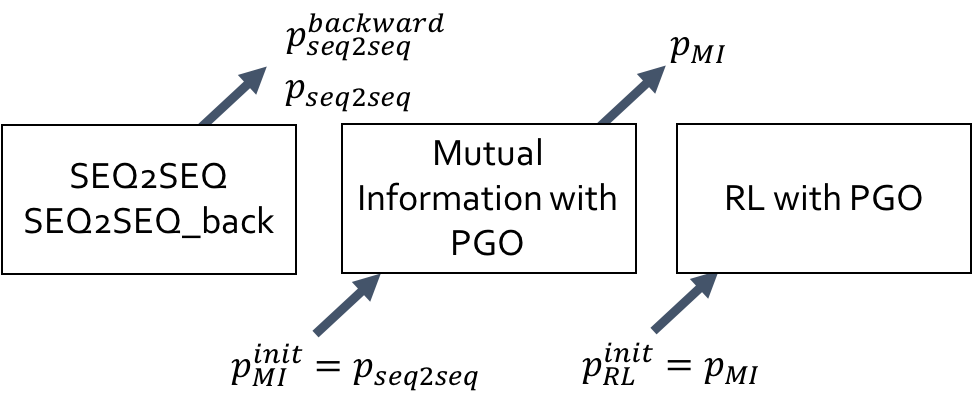
\includegraphics[width=0.4\textwidth]{three_steps.png} 
    \label{fig:three_steps}
    \caption{\small Training Procedure of the proposed Reinforcement Learning Model}
 \end{figure}
Any RL method falls into one of policy-based, value-based, or actor-critic RL areas. Among policy-based RL methods, a policy gradient optimization (PGO) using REINFORCE algorithm \cite{Williams} has been widely used. \cite{Li} also used the REINFORCE algorithm for learning the RL model. The training procedure of the RL model is divided into three steps as shown in the Fig.\ref{fig:three_steps}. First, we train a SEQ2SEQ model and a SEQ2SEQ backward model. Next, we train a mutual information model learned by PGO maximizing the semantic coherence (Eq.\ref{eq:reward3}). The policy parameters of the model are initialized by the parameters of the pre-trained SEQ2SEQ model, and its objective function is:
\begin{equation}
	J(\theta)= 	\mathbf{E} [m(\hat{a},[u_{t-1},u_t])]
\end{equation}
where $m(\hat{a},[u_{t-1},u_t])$ is equal to $r_{3,t}$ in the Eq.\ref{eq:reward3}. The gradient is estimated using the likelihood ratio trick in PGO:
\begin{equation}
	\nabla J(\theta) = m(\hat{a},[u_{t-1},u_t]) \nabla \log p_{RL}(\hat{a},[u_{t-1},u_t]) \label{eq:gradient}
\end{equation}

Then, we update the parameters in the encoder-decoder model using stochastic gradient ascent. In addition to the standard PGO method, \cite{Li} adopted a curriculum learning strategy proposed by \cite{Ranzato} and a baseline strategy. The baseline strategy is common in implementing PGO method since PGO tends to have high variance, and the strategy helps to reduce the variance.



\section{Experiment}

\begin{figure}[bt!]
    \centering
    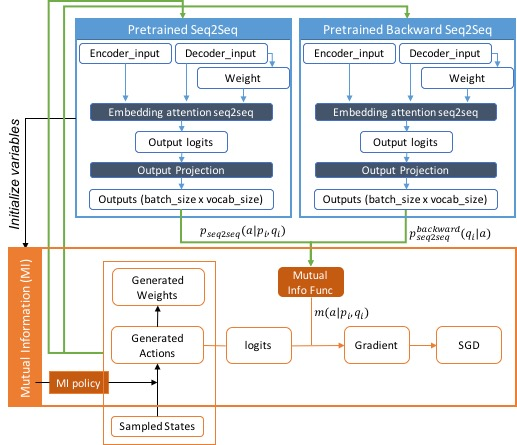
\includegraphics[width=0.48\textwidth]{mi_architecture} 
    \caption{\small SEQ2SEQ and MI model Code Architecture}
    \label{fig:mi_architecture}
 \end{figure}

\subsection{Dataset}
We first trained the modified SEQ2SEQ model on the CALLHOME American English Speech corpus (LDC97S42), consisting of 120 of 30-minute phone conversations between native English speakers.The size of vocabulary we used is 8038. However, in most of the conversation datasets, one speaker talks a long sentence or several sentences in a row and the other speaker answers with one or two words such as \textit{"mhm"},\textit{"okay"}, and \textit{"yeah"} as shown in Table.\ref{table:phone_data}. In fact, about 20\% of the utterances of the dataset is \textit{"mhm"}. As a results, the trained model after 44200 steps generated a short answer for long input utterances and a long answer for short input utterances (Table.\ref{table:phone_result}). Therefore, we concluded that this dataset may not have been appropriate for learning a dialog generation model.

Instead, we used the OpenSubtitles corpus (http://www.opensubtitles.org/) for both HRED and DRL. The OpenSubtitles corpus is a bilingual parallel corpus composed of movie subtitles. Originally constructed for machine translation, it has 20,400 files with 149.44 million tokens and 22.27 million sentence fragments. We used the 28 documents with English counterparts. The corpus is preprocessed by removing all ASCII symbols and adding consecutive speaker turns in an ad-hoc manner, that is to say we defaulted the first line in the script to be that of speaker one, the second line to be speaker two, and so on. Next, the corpus was normalized by case-folding, white space stripping, and converting all tokens to lower cases. Proper nouns and numbers were kept as is. 

with 50005 vocabulary size. The DRL paper also used this dataset, but unlike the paper, we didn't extract \textit{"i don't know what you are talking about"}. Instead, we refined abbreviated words such as \textit{"i'm"} $\rightarrow$ \textit{"i am"}, {"you're"} $\rightarrow$ \textit{"you are"}, {"i've"} $\rightarrow$ \textit{"i have"}, {"wanna"} $\rightarrow$ \textit{"want to"}, {"gonna"} $\rightarrow$ \textit{"going to"}, {"don't"} $\rightarrow$ \textit{"do not"}, etc. 

\begin{table}[t!]
    \centering
    \small
    \caption{\small Example Conversation in the CALLHOME corpus}
    \begin{tabular}{rl}
      \hline
        \textbf{A:} & who is in um someone not that they have problems but\\
        		    & someone who's like an okay student but kind of on the\\
        			& borderline you know like maybe not a great homelife\\
        			& and we would ha i got paired up\\
		\textbf{B:} & uh-huh \\
\textbf{A:} & with someone at um lipsmack i forget the school it was\\
			& actually in port richmond um breath i forget the name\\
			& of the school\\\
\textbf{B:} & really\\
\textbf{A:} & hensfiel no it was in the philadelphia school system and\\ 
			& it it was a middle school\\
\textbf{B:} & mhm\\
      \hline
    \end{tabular}
    \label{table:phone_data}
\end{table}

\subsection{Implementation}
Although it is not common to explain code structures in an academic paper, we explicitly mentioned functions and files in tensorflow we used as well as those written by us in this section.  
For the SEQ2SEQ model, we applied Sequence to sequence with attention mechanism and used GRU cells instead of LSTM cells. We used 3 layers and 512 units for all models. We implemented models in tensorflow version 1.0.1. We used \texttt{embedding\_attention\_seq2seq()} function in \texttt{seq2seq.py} and related functions/codes written in tensorflow. We also utilized \texttt{seq2seq\_model.py} in tensorflow version 0.12.x as a bottom line.\\
The \texttt{seq2seq\_model.py} is structured as follow (see Fig.\ref{fig:mi_architecture}): when the model is initialized, three main lists of placeholders are constructed - encoder, decoder, and weight. The length of the lists are encoder size, decoder size, and decoder size, respectively. Each element of a list is a tensor with a shape [batch size, None]. Variables are also built and initialized. In each step of training, batch size data are sampled in a given training dataset and converted into a proper format in the function \texttt{get\_batch()} by operations such as padding, adding GO id, sizing, etc. Then, these are fed to the placeholders. Output logits are computed through \texttt{embedding\_attention\_seq2seq()} function and losses are computed using a softmax loss function. Then, variables in the encoder-decoder recurrent neural network (RNN) are updated. \\
The mutual information model requires a pre-trained SEQ2SEQ model and a pre-trained backward SEQ2SEQ model for its initialization and for computing mutual information score. The model first builds three placeholder lists - concatenated states (e.g. $u_{t-1},u_t$), the most recent state (e.g. $u_t$) and weights for the backward model. Unlike SEQ2SEQ, only batch size number of states are sampled in each learning step. Then, actions are generated from the current RL policy given the sampled states. These states, actions, and weights are input to the pre-trained SEQ2SEQ and the pre-trained backward SEQ2SEQ model, and we obtain log probabilities from each model. Then, the mutual information score and the gradient in Eq.\ref{eq:gradient} are computed. According to the paper \cite{Li}, stochastic gradient descent (SGD) was applied to the objective function \ref{eq:obj_func}. However, since SGD is for minimization and the objective function has to be maximized, we used SGA instead to update variables of the encoder-decoder RNN.

\subsection{Results}
The training results of the backward SEQ2SEQ model after 109000 steps are presented in Table.\ref{table:backward_seq2seq}. Since it is a backward model, the bot generates the most likely utterance that will have the input utterance as its response. The examples in the Good section show good performance of the model. The generated responses in the Bad section do not make sense. The model tends to generate certain responses a lot such as "i am going to go to the bathroom", or to repeat all or some words in an input utterance. The training results of the SEQ2SEQ model with concatenated utterances after 107000 steps are presented in Table.\ref{table:seq2seq}. Each row of the table is one conversation, since the model consider two previous sentences. However, from the results, it was not hard to see that the model responses considering both two previous utterances. Also, it generates "i am sorry" or "no" many times. For example, for almost any human input utterance starting with "can you", it generates "no". \\
We wanted to see if the RL model were able to improve such dull response issues. We implemented only mutual information model without the curriculum strategy. However, during the decoding step after training, we found out that there might be an initialization problem due to the variable name feature since we use three models with a similar structure. Due to the time constraint, we were unable to solve the issue and present results in this paper. We hope we can solve the issue before the final presentation and will be able to add results in the final version of our final paper.

\begin{table}[bt!]
    \centering
    \small
    \caption{\small Backward Seq2Seq Model Examples}
    \begin{tabular}{c|rl}
    	\hline
      \hline
        & \textbf{human:} & i do not know man\\
		& \textbf{bot:} & what do you think\\		
& \textbf{human:} & that s amazing \\
& \textbf{bot:} & wow \\
& \textbf{human:} & that works best for me \\
& \textbf{bot:} & i will be right back \\
Good & \textbf{human:} & I love you too \\
& \textbf{bot:} & i love you \\
& \textbf{human:} & i know i am hot \\
& \textbf{bot:} & i am a little nervous \\
& \textbf{human:} & i am done with you \\
& \textbf{bot:} & i am a fucking bitch \\
\hline
& \textbf{human:} & i am going to go to the bathroom\\
& \textbf{bot:} & i am going to go to the bathroom \\
& \textbf{human:} & this is weird \\
& \textbf{bot:} & i am going to be a great man \\
Bad & \textbf{human:} & okay\\
& \textbf{bot:} & i am going to go to the bathroom\\
& \textbf{human:} & you look gorgeous \\
& \textbf{bot:} & i am going to go see the kitchen \\
& \textbf{human:} & fine\\
& \textbf{bot:} & i am fine\\
      \hline
    \end{tabular}
    \label{table:backward_seq2seq}
\end{table}

\begin{table}[bt!]
    \centering
    \small
    \caption{\small Seq2Seq Model Examples}
    \begin{tabular}{rl}
    	\hline
      \hline
        \textbf{human:} & this is bad \\
	\textbf{bot:} & this is a joke \\
	\textbf{human:} & what joke \\
	\textbf{bot:} & i do not know \\
	\textbf{human:} & what are you doing \\
	\textbf{bot:} & nothing \\
	\hline
	\textbf{human:} & you are a loser\\
	\textbf{bot:} & you are a real joke you know \\
	\textbf{human:} & what is a real joke \\
	\textbf{bot:} & i do not know \\
	\hline
	\textbf{human:} & how old are you \\
	\textbf{bot:} & eleven \\
	\textbf{human:} & you are so young boy \\
	\textbf{bot:} & i am sorry \\
	\textbf{human:} & it's totally okay \\
	\textbf{bot:} & i am sorry \\
	\textbf{human:} & what are you up to this weekend \\
	\textbf{bot:} & i am sorry \\
	\hline
	\textbf{human:} & where are you from \\
	\textbf{bot:} & where are you going \\
	\textbf{human:} & i am going home \\ 
	\textbf{bot:} & i am going to get you out of here \\
	\textbf{human:} & thank you but where \\
	\textbf{bot:} &  what is this \\
	\textbf{human:} & nothing \\
	\textbf{bot:} & i am sorry \\
      \hline
    \end{tabular}
    \label{table:seq2seq}
\end{table}

\section{Discussion}
In this project, we implemented HRED and DRL-SEQ2SEQ model with the OpenSubtitle Dataset. Unlike the results presented in the original paper of DRL-SEQ2SEQ \cite{Li}, our mutual information model generated poor responses and we could see that the model quickly diverges to wrong outcomes during training. There are several possible reasons for this poor performance. First, we didn't use curriculum strategy, but the strategy may play a critical role in RL learning since the reward functions do not perfectly describe quality of responses. Second, we used 0.5 for the learning rate of SGD (the default value in the tensorflow seq2seq model), but it may have been too large because the performance changed very quickly. Lastly, not using the baseline strategy may also have affected the performance since it is known that the strategy reduces the variance of PGO.
% include your own bib file like this:
%\bibliographystyle{acl}
%\bibliography{acl2017}
\bibliography{cis700}
\bibliographystyle{aaai}

\end{document}
